\documentclass[10pt, compress]{beamer}

\usetheme{m}

\usepackage{booktabs}
\usepackage[scale=2]{ccicons}
\usepackage{minted}
\usepackage{graphicx}
\usepackage{subfig}
\usepackage[export]{adjustbox}
\usepackage{physics}

\usepackage{layout}
\usepackage{printlen}
\usepackage{tcolorbox}

\usepackage[none]{hyphenat}

\usepackage{animate}

\usepackage{tikz}
\usetikzlibrary{arrows,positioning} 

\usemintedstyle{trac}

\title{Forward and Inverse Problems in Asteroseismology}
\subtitle{Main-Sequence Evolution of Solar-Like Stars}
\date{January 20, 2015}
\author{Earl Bellinger}
\institute{Solar System Seminar \\ 
Stellar Ages \& Galactic Evolution Group \\ 
Max-Planck-Institut f\"ur Sonnensystemforschung }

\begin{document}
\maketitle

\section{Overview}

\begin{frame}[fragile] \frametitle{Forward \& Inverse Problems}
    \begin{figure}
        \centering
        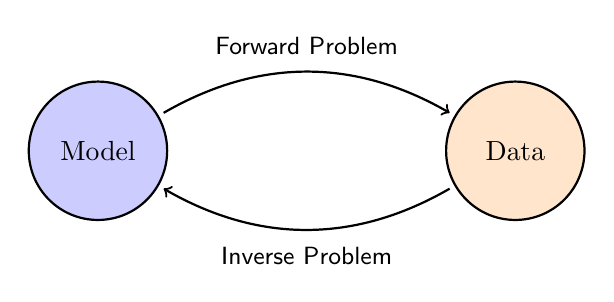
\begin{tikzpicture}[
        ->, 
        thick, 
        main node/.style={
            circle, 
            draw,
            minimum height=5em,
        },
        node distance=10em, 
        auto,
        pil/.style={
           thick,
           shorten <=2pt,
           shorten >=2pt
        }
    ]
    \node[main node, fill=blue!20!white] (model) {Model};
    \node[main node, right=of model, fill=orange!20!white] (data) {Data}
        %\draw[decoration={markings, mark=at position 1 with {\arrow[ultra thick]{>}}}, postaction={decorate}, bend left=30] %(model) to (data) 
        %node[above] {Forward Problem} (model);
        edge[pil, <-, bend right=30] node[above, yshift=0.1cm] {\sffamily\small{Forward Problem}} (model)
        edge[pil, ->, bend left=30] node[below, yshift=-0.1cm] {\sffamily\small{Inverse Problem}} (model);
\end{tikzpicture}

    \end{figure}
    
    \vspace{5mm}
    
    \only<2>{
    \begin{center}
        \begin{columns}
            \begin{column}{0.38\textwidth}
                \textbf{Linear forward problem}.
                \begin{equation}
                    d = Gm
                \end{equation}
            \end{column}
            \begin{column}{0.38\textwidth}
                \textbf{Linear inverse problem}.
                \begin{equation}
                    m = G^{-1}d
                \end{equation}
            \end{column}
        \end{columns}
    \end{center}}
\end{frame}

\begin{frame}[fragile] \frametitle{Examples} 
    \begin{tabular}{p{0.025\textwidth}|p{0.3\textwidth}|p{0.55\textwidth}} 
        \hline   & \textbf{Forward Problem} & \textbf{Inverse Problem} \\\hline\hline 
        1. & Simulate tracks of stellar \alert{evolution} & Determine the {\color{blue}initial conditions} and {\color{blue}evolutionary history} of a star from observations \\&&\\ 
        2. & Generate models of \alert{rotating} stars & Determine the {\color{blue}rotation profile} of an observed star from its $|m|>0$ modes \\&&\\ 
        3. & Generate models of stellar \alert{structure} & Determine the {\color{blue}structural profile} of an observed star from its oscillation frequencies \\\hline 
    \end{tabular}
\end{frame}

\begin{frame}[fragile] \frametitle{Why solve forward \& inverse problems?}
    \begin{figure}
        \centering
        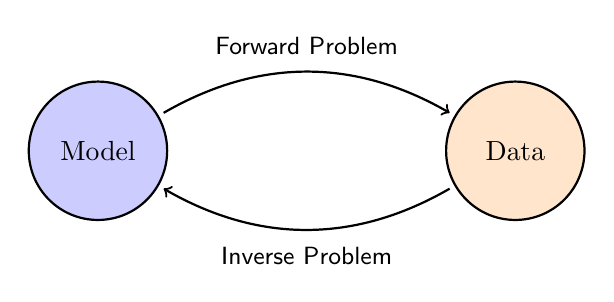
\begin{tikzpicture}[
        ->, 
        thick, 
        main node/.style={
            circle, 
            draw,
            minimum height=5em,
        },
        node distance=10em, 
        auto,
        pil/.style={
           thick,
           shorten <=2pt,
           shorten >=2pt
        }
    ]
    \node[main node, fill=blue!20!white] (model) {Model};
    \node[main node, right=of model, fill=orange!20!white] (data) {Data}
        %\draw[decoration={markings, mark=at position 1 with {\arrow[ultra thick]{>}}}, postaction={decorate}, bend left=30] %(model) to (data) 
        %node[above] {Forward Problem} (model);
        edge[pil, <-, bend right=30] node[above, yshift=0.1cm] {\sffamily\small{Forward Problem}} (model)
        edge[pil, ->, bend left=30] node[below, yshift=-0.1cm] {\sffamily\small{Inverse Problem}} (model);
\end{tikzpicture}

    \end{figure}
    
    \vspace{5mm}
    
    \textbf{Question}: Why do we want to solve forward and inverse problems? \\ \\
    \only<2>{\textbf{Answer}: Because they are awesome.}
\end{frame}

\begin{frame}[fragile] \frametitle{Awesome}
    \begin{figure}[!ht]
        \centering
        \subfloat[][]{
\includegraphics[width=.4\textwidth,frame]{figs/bear-punch.jpg}}\quad
        \subfloat[][]{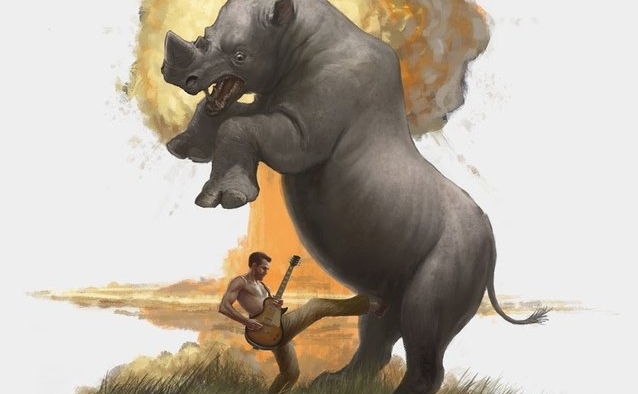
\includegraphics[width=.4\textwidth,frame]{figs/rhino.jpg}}\\
        \subfloat[][]{\includegraphics[width=.4\textwidth,frame]{figs/yngwie.png}}\quad
        \subfloat[][]{\includegraphics[width=.4\textwidth,frame]{figs/forward-inverse.png}}
        \caption{Things that are awesome}
    \end{figure}
\end{frame}

%%%%%%%%%%%%%%%%%%%%%%%%%%%%%%%%%%%%%%%%%%%%%%%%%%%%%%%%%%%%%%%%%%%%%%%%%%%%%%%%%%%%%%%%%%
%%% The forward problem %%%%%%%%%%%%%%%%%%%%%%%%%%%%%%%%%%%%%%%%%%%%%%%%%%%%%%%%%%%%%%%%%%
%%%%%%%%%%%%%%%%%%%%%%%%%%%%%%%%%%%%%%%%%%%%%%%%%%%%%%%%%%%%%%%%%%%%%%%%%%%%%%%%%%%%%%%%%%
\section{The forward problem}

\begin{frame}[fragile] \frametitle{Stellar evolution}
\end{frame}

\begin{frame}[fragile] \frametitle{Initial conditions}
    \begin{figure}[!hb] 
        \centering
        \noindent\makebox[\textwidth]{ 
            \subfloat[][Linear]{\includegraphics[width=.32\textwidth,frame]{figs/grid-linear.png}}\hfill
            \subfloat[][Random]{\includegraphics[width=.32\textwidth,frame]{figs/grid-random.png}}\hfill
            \subfloat[][Quasi-random]{\includegraphics[width=.32\textwidth,frame]{figs/grid-quasirandom.png}}
        }
        %\caption{A quasi-random grid of stellar models evolved from zero-age main sequence to near hydrogen exhaustion}
    \end{figure}
\end{frame}

\begin{frame}[fragile] \frametitle{Stellar pulsations}
    \begin{figure}[!hb] 
        \centering
        \animategraphics[
            autoplay, 
            autopause, 
            autoresume, 
            loop, 
            trim={2cm 0 2cm 0}, 
            width=.32\textwidth, 
            keepaspectratio]{30}{figs/anim_sph_harm/1_0/}{1}{39}
        \animategraphics[
            autoplay, 
            autopause, 
            autoresume, 
            loop, 
            trim={2.5cm 0 2.5cm 0}, 
            width=.32\textwidth, keepaspectratio]{15}{figs/anim_sph_harm/2_0/}{1}{39}
        \animategraphics[autoplay, autopause, autoresume, loop, trim={2cm 0 2cm 0}, width=.32\textwidth, keepaspectratio]{15}{figs/anim_sph_harm/3_0/}{1}{39}
        %\includegraphics[height=.75\textheight]{figs/sph_harm.png}
        \caption{Some solutions to Laplace's spherical harmonics $Y^m_\ell(\theta, \phi)$}
    \end{figure}
\end{frame}

\begin{frame}[fragile] \frametitle{Rank correlation testing}
    \begin{figure}[!hb] 
        %\centering
        \includegraphics[height=.85\textheight, trim={0 0 0 1cm}]{figs/corr-spearman-slides.pdf}
        %\caption{Spearman correlation coefficients between model variables and observables}
    \end{figure}
\end{frame}

\begin{frame}[fragile] \frametitle{Principal components analysis}
    \begin{figure}[!hb] 
        \centering
        \includegraphics[height=.875\textheight, trim={0 0 2cm 0}]{figs/corr-pca-slides.pdf}
        %\caption{Spearman correlation coefficients between model variables and principal components}
    \end{figure}
\end{frame}

%%%%%%%%%%%%%%%%%%%%%%%%%%%%%%%%%%%%%%%%%%%%%%%%%%%%%%%%%%%%%%%%%%%%%%%%%%%%%%%%%%%%%%%%%%
%%% The inverse problem %%%%%%%%%%%%%%%%%%%%%%%%%%%%%%%%%%%%%%%%%%%%%%%%%%%%%%%%%%%%%%%%%%
%%%%%%%%%%%%%%%%%%%%%%%%%%%%%%%%%%%%%%%%%%%%%%%%%%%%%%%%%%%%%%%%%%%%%%%%%%%%%%%%%%%%%%%%%%
\section{The inverse problem}

\begin{frame}[fragile] \frametitle{When can we solve an inverse problem?}
    \textbf{Definition}. {\color{blue} Well-posed problem} 
    \begin{enumerate}
        \item A solution exists
        \item The solution is unique
        \item The solution's behavior changes continuously with the initial conditions
    \end{enumerate} 
    \textbf{Reminder}. Linear inversion problem: $m=G^{-1}d$. \\ \\
    \pause \textbf{Question}. When can we invert a matrix? \\ \\
    \pause \textbf{Answer}. Only when the matrix is square and its determinant is 0. \\ And that's just a linear inversion problem! \\ 
    \begin{center} $\Rightarrow$
        Inverse problems are generally \alert{ill-posed}, and even when \\ they are not, they are often \alert{ill-conditioned}. 
    \end{center}
\end{frame}


\begin{frame}[fragile] \frametitle{Motivation: Classification}
    \begin{figure}
        \centering
        \includegraphics[height=.75\textheight,frame]{figs/classification.png}
        \caption{A typical linear classification problem}
    \end{figure}
\end{frame}

\begin{frame}[fragile] \frametitle{Motivation: Non-linear Classification}
    \begin{figure}
        \centering
        \includegraphics[height=.75\textheight,frame]{figs/classification-xor.png}
        \caption{The XOR Problem: a perceptron can only learn classes that are linearly separable}
    \end{figure}
\end{frame}


\begin{frame}[fragile] \frametitle{Thanks for your attention!}
    \begin{figure}[!hb] 
        \centering
        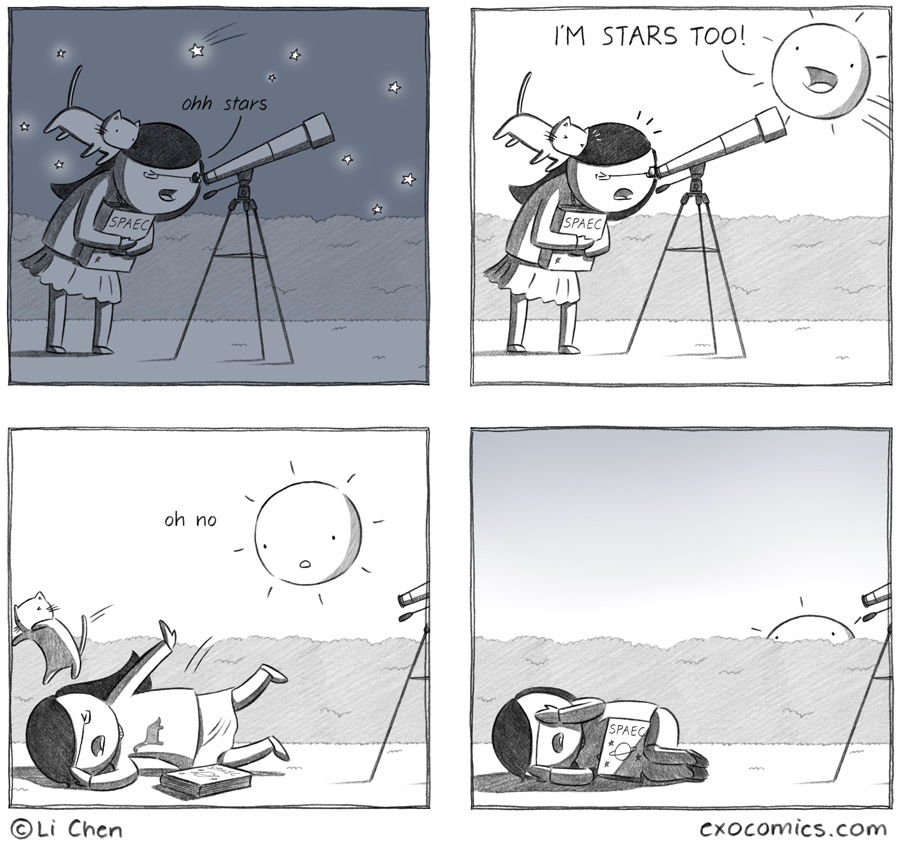
\includegraphics[height=.85\textheight,frame]{figs/comic.jpg}
    \end{figure}
\end{frame}


\end{document}
